\TODO

\begin{itemize}
    \item EHW
    \item POE
\end{itemize}

\section{Artificial Evolution}

\TODO

\begin{itemize}
    \item Antenna design
    \item Robot controllers
\end{itemize}

\subsection{Genetic Algoritmhs}

\TODO

\begin{itemize}
    \item Select, Cross, Mutate
    \item Genotype to Phenotype
\end{itemize}

\subsection{Evolution in Materio}

\TODO

\section{Artificial Development}

\TODO

\begin{itemize}
    \item Attractors
    \item Adaptation
    \item Graceful degradation
\end{itemize}

\subsection{Lindenmayer Systems}

\TODO

\section{Cellular Automata}

\TODO

\begin{itemize}
    \item 1D, 2D, 3D
    \item Neighborhoods
    \item Wolfram's classes
\end{itemize}

\section{FPGA}

\TODO

\section{PCI Express}

The PCI Express interface was designed to tackle the arising trouble with clocked parallel buses like PCI.
The problem with such buses is that the clock speed can not be increased beyond a given threshold, as the slightly different lengths of the wires causes data to arrive at slightly different times.
Reducing the clock period to less than the variation in arrival time means the data will become corrupted.
This problem is exacerbated with increasing bus size.

PCI Express is therefore based on serial communication over differential pairs (lanes\footnotemark) without the need for a reference clock \cite{pcie}.
\footnotetext{
    PCI Express operates in full duplex mode, which means that each lane has an independent differential pair in each direction.
    1, 2, 4, 8, 16 or 32 lanes are supported, but data is striped and thus still transmitted serially.
}
This allows an extremely fast clock speed compared to a parallel bus, and much greater bandwidth in total.
PCI Express consists of three layers; the physical layer, the data link layer and the transaction layer, structured as shown in \figurename~\ref{fig:pcie}.

\begin{figure}[!ht]
    \centering
    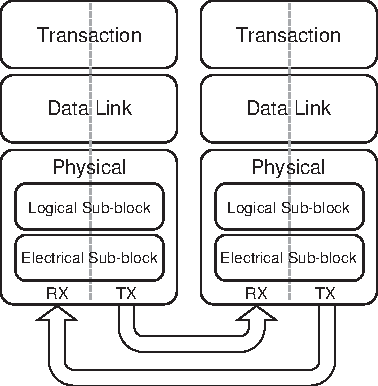
\includegraphics[width=0.5\textwidth]{pcie}
    \caption{High-level diagram showing the layered structure of PCI Express. (Reprinted from \cite{pcie})}
    \label{fig:pcie}
\end{figure}

The transaction layer's primary responsibility is the creation and parsing of transaction layer packets (TLPs).
TLPs are used to trigger events or start various transactions, most commonly to initiate read and write requests\footnotemark.
\footnotetext{
    Read and write requests are directed at one of up to six base address registers (BARs).
    They represent internal memory areas that can be anywhere from a few bytes to several gigabytes in size.
}
Most requests entail the return of a completion TLP containing the requested data or other information.
TLPs consists of multiple 32-bit double words (DW), where the first is a common header describing the type of packet.

The data link layer ensures integrity by adding error detection codes to outgoing TLPs and performing error detection and correction on incoming TLPs.
It is also responsible for retransmission if corruption occurs.

The physical layer is responsible for serialization and deserialization of the data stream.
Each byte is padded with two extra bits (8b/10b encoding) to allow clock recovery.

\section{Related Work}

\TODO

\subsection{CAM-Brain Machine}

\TODO

\subsection{CAM-8}

\TODO
